\documentclass[a4paper,12px]{article}

\usepackage{graphicx}
\usepackage[english]{babel}
\usepackage{fancyhdr}
\usepackage{lastpage}
\usepackage{xifthen}
\usepackage[linesnumberedhidden, titlenotnumbered]{algorithm2e}
\usepackage{lipsum}
\usepackage{hyperref}
\usepackage{array}
\usepackage{tabularx}

\usepackage{minted}
\usepackage{caption}
\usepackage{amssymb}

\pagestyle{fancy}
\lhead{
\includegraphics[width=7cm]{logoUvA}}
\rhead{\footnotesize \textsc {Report\\ \opdracht}}
\lfoot
{
    \footnotesize \studentA
    \ifthenelse{\isundefined{\studentB}}{}{\\ \studentB}
    \ifthenelse{\isundefined{\studentC}}{}{\\ \studentC}
    \ifthenelse{\isundefined{\studentD}}{}{\\ \studentD}
    \ifthenelse{\isundefined{\studentE}}{}{\\ \studentE}
}
\cfoot{}
\rfoot{\small \textsc {Page \thepage\ of \pageref{LastPage}}}
\renewcommand{\footrulewidth}{0.5pt}

\fancypagestyle{firststyle}
{
    \fancyhf{}
    \renewcommand{\headrulewidth}{0pt}
    \chead{
\includegraphics[width=7cm]{logoUvA}}
    \rfoot{\small \textsc {Page \thepage\ of \pageref{LastPage}}}
}

\setlength{\topmargin}{-0.3in}
\setlength{\textheight}{630pt}
\setlength{\headsep}{40pt}

% =================================== DOC INFO ===================================

\newcommand{\titel}{Surface approximation}
\newcommand{\opdracht}{Python Assignment 1}
\newcommand{\docent}{Dr. A.J.P. Heck}
\newcommand{\cursus}{Numerical Recipes Project}
\newcommand{\vakcode}{5062NURP6Y}
\newcommand{\datum}{\today}
\newcommand{\studentA}{Robin Klusman}
\newcommand{\uvanetidA}{10675671}
\newcommand{\studentB}{Maico Timmerman}
\newcommand{\uvanetidB}{10542590}
%\newcommand{\studentC}{Boudewijn Braams}
\newcommand{\uvanetidC}{10401040}
%\newcommand{\studentD}{Govert Verkes}
\newcommand{\uvanetidD}{10211748}
%\newcommand{\studentE}{Naam student 5}
\newcommand{\uvanetidE}{UvAnetID student 5}

% ===================================  ===================================

\begin{document}
\thispagestyle{firststyle}
\begin{center}
    \textsc{\Large \opdracht}\\[0.2cm]
    \rule{\linewidth}{0.5pt} \\[0.4cm]
    {\huge \bfseries \titel}
    \rule{\linewidth}{0.5pt} \\[0.2cm]
    {\large \datum  \\[0.4cm]}

    \begin{minipage}{0.4\textwidth}
        \begin{flushleft}
            \emph{Student:}\\
            {\studentA \\ {\small \uvanetidA \\[0.2cm]}}
            \ifthenelse{\isundefined{\studentB}}{}{\studentB \\ {\small \uvanetidB \\[0.2cm]}}
            \ifthenelse{\isundefined{\studentC}}{}{\studentC \\ {\small \uvanetidC \\[0.2cm]}}
            \ifthenelse{\isundefined{\studentD}}{}{\studentD \\ {\small \uvanetidD \\[0.2cm]}}
            \ifthenelse{\isundefined{\studentE}}{}{\studentE \\ {\small \uvanetidE \\ [0.2cm]}}
        \end{flushleft}
    \end{minipage}
    ~
    \begin{minipage}{0.4\textwidth}
        \begin{flushright}
            \emph{Supervisor:} \\
            \docent \\[0.2cm]
            \emph{Course:} \\
            \cursus \\[0.2cm]
            \emph{Course code:} \\
            \vakcode \\[0.2cm]
        \end{flushright}
    \end{minipage}\\[1 cm]
\end{center}


% =================================== FRONT PAGE ===================================

\vspace{2cm}
\begin{center}
    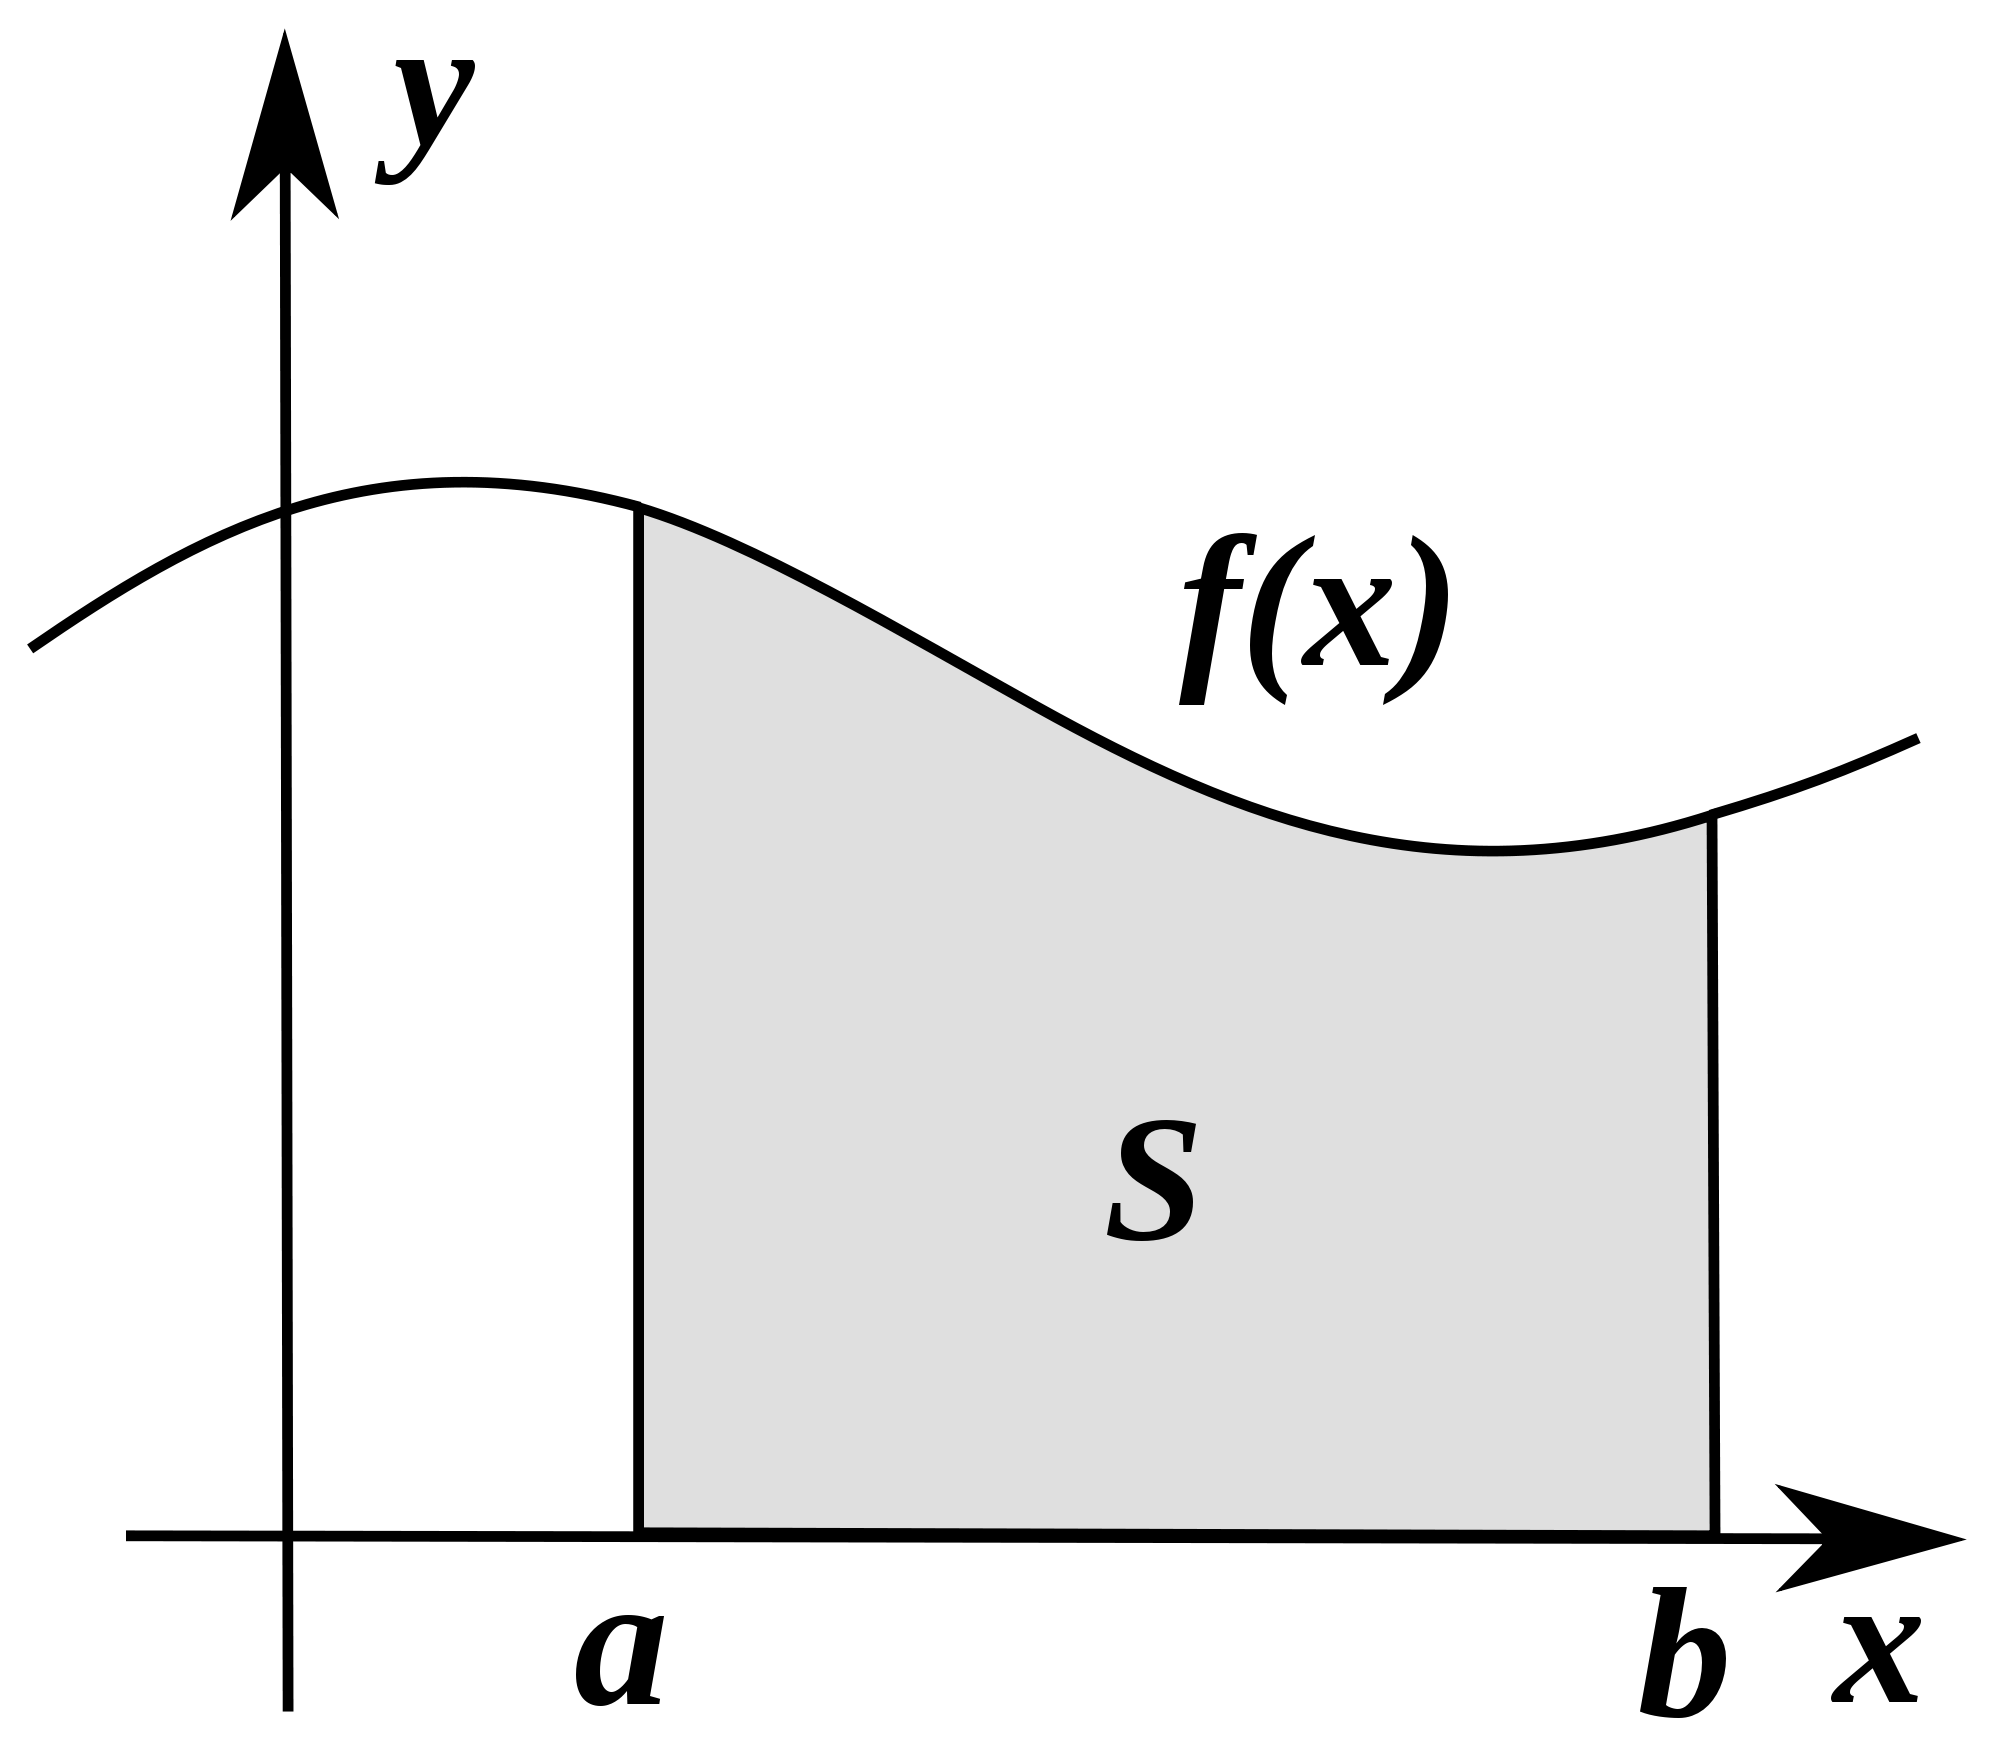
\includegraphics[width=(\textwidth/5*3)]{curve}
\end{center}
\clearpage

\tableofcontents
\vspace{5mm}

% =================================== MAIN TEXT ===================================

\section{Riemann}

The Riemann sum is approximation is relatively simple. The interval $[a,b]$ in
which the surface area under a curve needs to be determined is divided into $n$
subintervals. For each of these subintervals we take either the value of $f(x)$
for the left bound, right bound or center of that subinterval. Then we multiply
the value of $f(x)$ by the width of the subinterval.

In our implementation of the Riemann sum method we use a function that takes a
function $f$, the left bound $a$, the right bound $b$, the amount of
subintervals $n$, and the method as arguments. We then use a loop from $i=0$ to
$i=n-1$ so that we take exactly $n$ subintervals. The $x$ values of the left,
center and right bound methods are then determined by $x=a+i*h$, $x=a+(i+0.5)*h$
and $x=a+(i+1)*h$ respectively. We then calculate the value of $f(x)$ for this
$x$ and multiply that value by $h$ to get the surface area of the rectangle
underneath the curve. The absolute value of $f(x)$ is used so (partly) negative
functions also result in a correct surface area.

The surface areas of all these rectangles are then summed to get an
approximation of the total surface area underneath the curve.

\section{Trapezoid}

The Trapezoid rule approximation is a bit more complicated and also a bit more
accurate than the Riemann sum. The function again takes the same arguments
discussed in the Riemann section, but without the method. Then instead of
calculating the surface area of a rectangle made with a single value $f(x)$
now a trapezoid made with two values, $f(x_k)$ and $f(x_{k+1})$ is used to
calculate the surface area of the subintervals.

The implementation of the Trapezoid rule does not differ much from the Riemann
sum one. Instead of calculating a single value for $x$ per iteration we now
determine two values, $x_k$ and $x_{k+1}$ with $x_k=a+i*h$ and
$x_{k+1}=a+(i+1)*h$. With these two values we can simply determine the surface
area of a trapezoid underneath the curve with $S=(f(x_k)+f(x_{k+1})*(h/2)$. We
again use the absolute values of $f(x)$ so also (partly) negative functions can
be used.

The surface area of all these trapezoids is then summed to approximate the total
area underneath the curve in a slightly more accurate way than the Riemann sum
does.

\section{Simpson}

The Simpson rule approximation finds the surface area in a subinterval by
finding a curve through three points on the actual curve of $f$, $x_k$,
$x_{k+1}$ and $x_{k+2}$. Then the equation of this
curve is found using Lagrange-interpolation and the surface area underneath it
can be determined through regular integration using the primitive function.

The implementation of this method again takes the same arguments as the trapezoid
method. Only now the number of iterations is halved, because we need a total of
three points, $x_k$, $x_{k+1}$ and $x_{k+2}$. In the next iteration $x_k$
becomes the $x_{k+2}$ of the previous iteration. The values for $x_{k+j}$ are
found by $x_{k+j}=a+(i+j)*h$. We then determine the surface area under these
sub-curves by $S=(f(x_k) + 4f(x_{k+1}) + f(x_{k+2}))*(h/3)$. As with all
previous methods the absolute value of $f(x)$ is used to also accommodate
negative functions.

Summing the surface area under all these sub-curves results in an approximation
of the actual surface area under $f$.

\section{Monte Carlo}

The Monte Carlo method is quite different from all previous methods. Instead of
using a sum of sub-areas, the surface underneath the curve is approximated by
plotting points at random within a rectangle. This rectangle must span exactly
$[a,b]$ on the x-axis and span at least $[0,y_{max}]$ on the y-axis. $y_{max}$
is defined as the maximum value of $f(x)$ within $[a,b]$. We then determine the
fraction of points that is below the curve and multiply that by the total
surface area of the rectangle to find to approximate surface area. The more
points that are plotted the more accurate this approximation becomes.

In this implementation we again use the same arguments as before, only now $n$
has a different purpose. In this case $n$ is the number of points we plot
instead of the number of sub-intervals. First the value of $y_{max}$ needs to be
determined so that we can define a rectangle large enough to fit $f(x)$. This is
done by using a loop that checks the values of $f(x)$ with a step size of 0.01.
We chose to use 0.01 to make sure we don't miss any small peaks. Then just to be
sure we round the value of $y_{max}$ up to the nearest integer value and add 1
to it.  Now we can say with relative certainty that $y_{max}$ is indeed larger
than the maximum value of $f$ within the interval. After this is determined
points need to be plotted in this rectangle and we need to keep track of whether
or not these points are below or above the curve of $f$. When all points are
plotted we determine the fraction of points that is under the curve with
$fraction = p_{below}/(p_{below}+p_{above})$.

Finally this fraction is multiplied by the surface area of the rectangle to find
an approximation of the surface area under $f$.


\section{Efficiency}

% =================================== REFERENCES ===================================

%\clearpage
%\bibliographystyle{unsrt}
%\bibliography{bib}

\end{document}
